\subsubsection{Séquentiel}
L'opérateur séquentiel, aussi abrégé {\em S} dans Taggre, est un opérateur très simple.
%
Son but est de fusionner les tâches qui n'apportent pas de parallélisme, elles ne font qu'ajouter du surcoût d'ordonnancement au temps total de la simulation.
%
En agrégeant ces tâches ensemble, on ne perd pas de parallélisme et on économise le temps d'ordonnancement des tâches.
%
On peut reconnaître un groupe de deux tâches séquentielles par le fait qu'une des tâches n'a qu'un seul successeur et l'autre tâche n'a qu'un seul prédécesseur (Fig~\ref{fig:algo_S}).


%   (-_-)   %
\begin{figure}[t!]
  \centering
  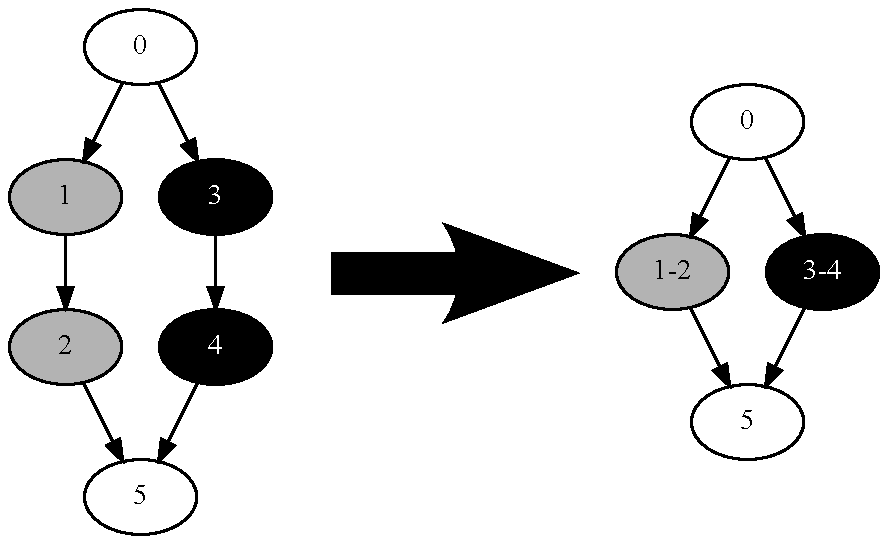
\includegraphics[width=0.6\textwidth]{algo_S}
  \caption{Exemple d'agrégation par l'opérateur séquentiel.}
  \label{fig:algo_S}
\end{figure}

\begin{algorithm}
  \KwData{DAG}
  {\sc Taches} = liste vide \\
  mettre les tâches de DAG dans {\sc Taches} \\
  \While{{\sc Taches} n'est pas vide} {
    {\sc T1} = retirer le premier de {\sc Taches} \\
    \If{Le nombre de successeurs de {\sc T1} == 1} {
      {\sc T2} = premier successeur de {\sc T1} \\
      \If{Le nombre de prédécesseurs de {\sc T2} == 1} {
        agréger {\sc T1} et {\sc T2}\\
      }
    }
  }
  \caption{Algorithme de l'opérateur séquentiel.}
  \label{algo:algo_S}
\end{algorithm}
